%
%
%
%\VignetteIndexEntry{CummeRbund User Guide}
%\VignetteKeywords{cummeRbund,visualization,NGS,sequencing,cufflinks,cuffdiff}
%\VignettePackage{cummeRbund}
%
%%%%%%%%%%%%%%%%%%%%%%%%%%%%%%%%%%%%%%%%%%%%%%%%%%%%%%%%%%%%%%%%%%%%%%%%%%%

\documentclass[10pt]{article}
\usepackage[margin=0.75in]{geometry}
\usepackage{amsmath}
\usepackage[authoryear,round]{natbib}
\usepackage{hyperref}
\usepackage{graphicx, subfig}
\hypersetup{
    colorlinks,
    citecolor=black,
    filecolor=black,
    linkcolor=red,
    urlcolor=black
}
\usepackage{theorem}
\usepackage{float}
\usepackage{ifthen}
\usepackage[OT1]{fontenc}

%%%%%%
% Alter some LaTeX defaults for better treatment of figures:
    % See p.105 of "TeX Unbound" for suggested values.
    % See pp. 199-200 of Lamport's "LaTeX" book for details.
    %   General parameters, for ALL pages:
    \renewcommand{\topfraction}{0.9}	% max fraction of floats at top
    \renewcommand{\bottomfraction}{0.8}	% max fraction of floats at bottom
    %   Parameters for TEXT pages (not float pages):
    \setcounter{topnumber}{2}
    \setcounter{bottomnumber}{2}
    \setcounter{totalnumber}{4}     % 2 may work better
    \setcounter{dbltopnumber}{2}    % for 2-column pages
    \renewcommand{\dbltopfraction}{0.9}	% fit big float above 2-col. text
    \renewcommand{\textfraction}{0.07}	% allow minimal text w. figs
    %   Parameters for FLOAT pages (not text pages):
    \renewcommand{\floatpagefraction}{0.7}	% require fuller float pages
	% N.B.: floatpagefraction MUST be less than topfraction !!
    \renewcommand{\dblfloatpagefraction}{0.7}	% require fuller float pages

	% remember to use [htp] or [htpb] for placement
%%%%%%%%%%%



\newcommand{\R}{{\textsf{R}}}
\newcommand{\code}[1]{{\texttt{#1}}}
\newcommand{\term}[1]{{\emph{#1}}}
\newcommand{\Rpackage}[1]{\textsf{#1}}
\newcommand{\Rfunction}[1]{\texttt{#1}}
\newcommand{\Robject}[1]{\texttt{#1}}
\newcommand{\Rclass}[1]{{\textit{#1}}}
\newcommand{\Rmethod}[1]{{\textit{#1}}}
\newcommand{\Rfunarg}[1]{{\textit{#1}}}

\bibliographystyle{plainnat}
\title{CummeRbund: Visualization and Exploration of Cufflinks High-throughput Sequencing Data}

\author{Loyal A. Goff, Cole Trapnell, David Kelley}
\date{September 24, 2012}
\usepackage{Sweave}
\begin{document}

\maketitle
\tableofcontents
\clearpage
\section{Requirements}
NOTE: cummeRbund 2.0 was designed in conjunction with the release of cufflinks 2.0.  While we attempted to preserve backwards-compatability, it is highly recommended
that you update your cufflinks version >=2.0 to take full advantage of the improvements in modeling, reporting, and visualization that have been incorporated. 
\begin{itemize}
	\item Cufflinks $\ge$ v2.0.0
	\item SQLite 
	\item R $\ge$ v2.7.0
	\item Packages:
	\begin{itemize}
		\item \Rpackage{RSQLite}
		\item \Rpackage{ggplot2 v0.9.2}
		\item \Rpackage{reshape2}
		\item \Rpackage{plyr}
		\item \Rpackage{fastcluster}
        \item \Rpackage{rtracklayer}
        \item \Rpackage{Gviz}
		\item Recommended:
		\begin{itemize}
			\item \Rpackage{Hmisc}
		\end{itemize}
	\end{itemize}
\end{itemize}
	
\clearpage

\section{Introduction}
	\Rpackage{cummeRbund} is a visualization package for Cufflinks high-throughput sequencing data. It is designed to help you navigate through the large amount of data produced from a Cuffdiff RNA-Seq differential expression
	analysis. The results of this analysis are typically a large number of inter-related files that are not terribly intuitive to navigate through. cummeRbund helps promote rapid analysis of RNA-Seq data by aggregating, indexing,
	and allowing you easily visualize and create publication-ready figures of your RNA-Seq data while maintaining appropriate relationships between connected data points.
	CummeRbund is a multifaceted suite for streamlined analysis and visualization of massively parallel RNA differential expression data sequencing data. 
	
	CummeRbund begins by re-organizing output files of a cuffdiff analysis, and storing these data in a local SQLite database. CummeRbund indexes the data to speed up access to specific feature data (genes, isoforms, TSS, CDS, etc.),
	and preserves the various relationships between these features. Access to data elements is managed via the RSQLite package and data are presented in appropriately structured R classes with various convenience functions designed
	to streamline your workflow. This persistent database storage means that inter-connected expression values are rapidly accessible and quickly searchable in future analyses.
	
	CummeRbund defines two types of data classes, 'pointer' or reference classes describe SQL connections to the database without directly containing data, and 'data' classes that retrieve a subset of related data points such as associated
	features from a given gene or gene set. Each class type has methods for direct access to FPKM vales, differential expression information, statistical test results, raw and normalized fragment counts, individual replicate FPKM values, and additional annotation information for features. Output formats allow 
	for browsing and analysis of data in standard R objects (data.frame, list, etc). CummeRbund was designed to provide analysis and visualization tools analogous to microarray data. In this regard, numerous plotting methods are provided for visualization 
	of RNA-Seq data quality and global statistics, and simple routines for plotting expression levels for one or thousands of genes, their isoforms, TSS groups, or CDS groups.
	  
	The base class, \Rclass{cuffSet} is a 'pointer' to cuffdiff data that are stored out-of-memory in a sqlite database.

\clearpage

\section{CummeRbund Classes}

\subsection{CuffSet Class}
	A pointer class to control access to the sqlite tables holding the Cufflinks data. The primary slot is DB which contains the RSQLite connection object. This can be accessed using the \Rmethod{DB()} accessor.
	The additional slots (genes, isoforms, TSS, and CDS) are each instances of the \Rclass{CuffData} class and are pointers to sets of tables for each data subtype. They can be accessed with similar accessor wrappers.
	This is the default class created by \Rmethod{readCufflinks}.  By default, \Rclass{CuffData} accessor methods applied to a \Rclass{CuffSet} class will operate on the 'genes' slot. The \Rmethod{runInfo()} method can be used to retrieve information about
	the actual cuffdiff run itself, including command-line arguments used to generate the results files.

\subsection{CuffData Class}
	The \Rclass{CuffData} class is also a pointer class to the SQL backend, but each instance is specific for a data subtype (genes, isoforms, TSS, CDS). Again, there is an DB slot (accessible using \Rmethod{DB()}) that contains the RSQLite connection object.
	There are several accessor, setter, and plotting methods that allow for global analysis of all features within a \Rmethod{CuffData} class.Subsetting is currently being re-written, however, it is primarily done through the 'gene\_id' field.
	Available slots for the CuffData class are: 
	\begin{itemize}
		\item DB: RSQLite connection object
		\item tables: A \Rclass{list} of tables in the SQLite DB that contain the cufflinks data.
		\item filters: A \Rclass{list} of filters for subsetting (not implemented yet).
		\item type: A \Rclass{character} field describing the data (ie. 'genes','isoforms','TSS','CDS','other')
		\item idField: The name of the identifying index field for this object (eg. 'gene\_id' for type='gene', or 'isoform\_id' for type='isoform')
	\end{itemize}
	Making the best use of either the CuffSet or CuffData classes will enable you to keep the entire dataset out of memory and significantly improve performance for large cufflinks datasets.

\subsection{CuffDist Class}
	The \Rclass{CuffDist} class is an pointer class that contains the results of the various 'distribution tests' performed by cuffdiff.  These include differential promoter usage, differential splicing, and differential CDS usage.  These are independent tests from the differential analysis of gene-, isoform-, TSS-, and CDS-level features and therefore
	have their own container type to distinguish them as such.  The 'promoters', 'relCDS', and 'splicing' slots of a \Rclass{CuffSet} class are all \Rclass{CuffDist} instances.
	
	Available slots for the CuffDist class are:
	\begin{itemize}
	\item DB: RSQLite connection object
		\item tables: A \Rclass{list} of tables in the SQLite DB that contain the distribution test data.
		\item type: A \Rclass{character} field describing the data (ie. 'promoters','relCDS','splicing')
		\item idField: The name of the identifying index field for this object (eg. 'TSS\_group\_id' for type='promoters', or 'CDS\_id' for type='relCDS', etc.)
	\end{itemize}

\subsection{CuffFeatureSet Class}
	The \Rclass{CuffFeatureSet} class is a data-storage container that holds all available data for a pre-determined list of features. Slots for FPKM data, differential regulation data, and feature-level annotation are all available. Unlike the previous classes, this class contains no connection information to the SQL database, but
	rather contains several slots with \Rclass{data.frame} objects storing multiple-features worth of information.  There are available accessors, and plotting methods that are designed to present multiple-features worth of information (eg. heatmaps, scatterplots, etc)
	Available slots for a \Rclass{CuffFeatureSet} object include:
	\begin{itemize}
		\item annotation: Holds all feature-level annotation information for all features in object.
		\item fpkm: A data frame of FPKM data across all conditions, for all features in object.
		\item repFpkm: A data frame of deconvolved FPKM values across individual replicates, for all features in object.
		\item diff: A data frame of differential expression/regulation data for all features in object.
		\item count: A data frame containing raw and normalized fragment counts, variance, dispersion, and uncertainty for all features in object.
        \item genome: A character string indicating which build of the genome
        the associated features are derived from.  (e.g. `hg19',`mm9')
	\end{itemize}
	
	A specialized sub-class of \Rclass{CuffFeatureSet} is the \Rclass{CuffGeneSet} class. This subclass adds additional slots to contain all isoforms, TSS, and CDS information for a given set of gene\_ids.  The \Rclass{CuffGeneSet} class is designed to aggregate all relevant
	information for a set of genes into one object for easy analysis and/or manipulation.
	The \Rclass{CuffGeneSet} object adds the following slots:
	\begin{itemize}
		\item ids: A 'character' list of all gene\_ids used in object.
		\item isoforms: A \Rclass{CuffFeatureSet} object for all isoforms of genes in object.
		\item TSS: A \Rclass{CuffFeatureSet} object for all TSS of genes in object.
		\item CDS: A \Rclass{CuffFeatureSet} object for all CDS of genes in object.
	\end{itemize}

\subsection{CuffFeature Class}
	The \Rclass{CuffFeature} class is designed for single-feature-level data analysis and plotting.  The methods available for this object are designed to analyze or visualize information about a specific feature.
	This is a 'data' object, as opposed to a 'pointer' object to the database backend. There is a validity requirement that a \Rclass{CuffFeature} object only point to data from a single feature.
	Available slots for a \Rclass{CuffFeature} object include:
	\begin{itemize}
		\item annotation: Holds feature-level annotation information for a given feature.
		\item fpkm: A data frame of FPKM data across all samples for a given feature.
		\item repFpkm: A data frame of deconvolved FPKM values across all replicates for a given feature.
		\item diff: A data frame of differential expression/regulation data for a given feature.
		\item count: A data frame containing raw and normalized fragment counts, variance, dispersion, and uncertainty for a given feature.
	\end{itemize}
	
	A specialized sub-class of \Rclass{CuffFeature} is the \Rclass{CuffGene} class. This subclass adds additional slots to contain all isoform, TSS, and CDS information for a given gene.
	The \Rclass{CuffGene} object adds the following slots:
	\begin{itemize}
		\item id: The common 'gene\_id' for all data in object
		\item isoforms: A \Rclass{CuffFeature} object for all isoforms of a given gene.
		\item TSS: A \Rclass{CuffFeature} object for all TSS of a given gene.
		\item CDS: A \Rclass{CuffFeature} object for all CDS of a given gene.
        \item features: A \Rclass{data.frame} object containing feature
        information for the transcript models describing the gene.
	\end{itemize}

\clearpage

\section{Reading cuffdiff output}
\Rpackage{cummeRbund} was designed to process the multi-file output format for a 'cuffdiff' differential expression analysis.  In this type of analysis, a user will use a reference .gtf file (either known annotation or a .gtf file created from a cufflinks assembly or merge of assemblies) and quantitate the expression values and differential regulation of the annotation(s) in the .gtf file across two or more SAM/BAM files.
By design, cuffdiff produces a number of output files that contain test results for changes in expression at the level of transcripts, primary transcripts, and genes. It also tracks changes in the relative abundance of transcripts sharing a common transcription start site, and in the relative abundances of the primary transcripts of each gene. Tracking the former allows one to see changes in splicing, and the latter lets one see changes in relative promoter use within a gene. \\

Note:Early versions of Cuffdiff required that transcripts in the input GTF be annotated with certain attributes in order to look for changes in primary transcript expression, splicing, coding output, and promoter use. This is no longer the case with >=v1.1.1 of \Rpackage{cummeRbund}, however we still recommend the use of both the following attributes in your GTF file to enable all downstream features of \Rpackage{cummeRbund}. \\

These attributes are:
\begin{itemize}
	\item tss\_id: The ID of this transcript's inferred start site. Determines which primary transcript this processed transcript is believed to come from. Cuffcompare appends this attribute to every transcript reported in the .combined.gtf file.
	\item p\_id	The ID of the coding sequence this transcript contains. This attribute is attached by Cuffcompare to the .combined.gtf records only when it is run with a reference annotation that include CDS records. Further, differential CDS analysis is only performed when all isoforms of a gene have p\_id attributes, because neither Cufflinks nor Cuffcompare attempt to assign an open reading frame to transcripts.
\end{itemize}

cuffdiff calculates the FPKM of each transcript, primary transcript, and gene in each sample. Primary transcript and gene FPKMs are computed by summing the FPKMs of transcripts in each primary transcript group or gene group. The results are output in FPKM tracking files, the structure of which can be found in the cufflinks manual.\\

There are four FPKM tracking files:
\begin{itemize}
	\item \emph{isoforms.fpkm\_tracking}	Transcript FPKMs
	\item \emph{genes.fpkm\_tracking}	Gene FPKMs. Tracks the summed FPKM of transcripts sharing each gene\_id
	\item \emph{cds.fpkm\_tracking}	Coding sequence FPKMs. Tracks the summed FPKM of transcripts sharing each p\_id, independent of tss\_id
	\item \emph{tss\_groups.fpkm\_tracking}	Primary transcript FPKMs. Tracks the summed FPKM of transcripts sharing each tss\_id
\end{itemize}

cuffdiff also performs differential expression tests between supplied conditions. This tab delimited file lists the results of differential expression testing between samples for spliced transcripts, primary transcripts, genes, and coding sequences. For detailed file structure see cufflinks manual. \\

Four .diff files are created:
\begin{itemize}
	\item \emph{isoform\_exp.diff}	Transcript differential FPKM.
	\item \emph{gene\_exp.diff}	Gene differential FPKM. Tests difference sin the summed FPKM of transcripts sharing each gene\_id
	\item \emph{tss\_group\_exp.diff}	Primary transcript differential FPKM. Tests differences in the summed FPKM of transcripts sharing each tss\_id
	\item \emph{cds\_exp.diff}	Coding sequence differential FPKM. Tests differences in the summed FPKM of transcripts sharing each p\_id independent of tss\_id
\end{itemize}

In addition, cuffdiff also performs differential splicing, CDS usage, and promoter usage tests for each gene across conditions:

\begin{itemize}
	\item \emph{splicing.diff}	Differential splicing tests.
	\item \emph{CDS.diff}	Differential coding output.
	\item \emph{promoters.diff}	Differential promoter use.
\end{itemize}

All of these output files are related to each other through their various tracking\_ids, but parsing through individual files to query for important result information requires both a good deal of patience and a strong grasp of command-line text manipulation. Enter cummeRbund, an R solution to aggregate, organize, and help visualize this multi-layered dataset. \\
One of the principle benefits of using cummeRbund is that data are stored in a SQLite database.  This allows for out-of-memory analysis of data, quick retrieval, and only a one-time cost to setup the tables. By default, cummeRbund assumes that all output files from cuffdiff are in the current working directory.
To read these files, populate the 'cuffData.db' database backend, and return the \Rclass{CuffSet} pointer object, you can do the following. 

\begin{Schunk}
\begin{Sinput}
> library(cummeRbund)
\end{Sinput}
\end{Schunk}
%%fileDir<-("../../extdata/")

\begin{Schunk}
\begin{Sinput}
> cuff<-readCufflinks()
\end{Sinput}
\end{Schunk}

\begin{Schunk}
\begin{Sinput}
> cuff
\end{Sinput}
\begin{Soutput}
CuffSet instance with:
	 3 samples
	 400 genes
	 1203 isoforms
	 662 TSS
	 906 CDS
	 1062 promoters
	 1986 splicing
	 990 relCDS
\end{Soutput}
\end{Schunk}

Again, by default $dir$ is assumed to be the current working directory and \code{cuff<-readCufflinks()} should work if all appropriate files are in the current working directory. We now also
recommend that you use both the \Rfunarg{genome} and \Rfunarg{gtfFile} arguments to readCufflinks(). This will allow cummeRbund to archive the transcript structure information located in the .gtf file associated with
your particular cuffdiff run, as well as associate these transcripts with an appropriate genome build (e.g. 'hg19', 'mm9', etc) so as to allow for transcript-level visualizations and future integration with other external resources. 
Should you need to rebuild the SQLite backend for any reason, you can add the option \Rfunarg{rebuild=T} to \Rmethod{readCufflinks}.  Once the database is created, \Rmethod{readCufflinks} will default to using the SQL backend and should not need to rebuild this database.
Each R session should begin with a call to \Rmethod{readCufflinks} so as to initialize the database connection and create an object with the appropriate RSQLite connection information. 

\subsection{Adding additional feature annotation}
Gene- or feature-level annotation can be permanently added to the database tables for future querying. If you have a data.frame where the first column contains the 'tracking\_id' (eg. 'gene\_id' for genes, 'isoform\_id' for isoforms, etc). You can easily add feature level annotation using the \Rfunction{addFeatures()} function:

\begin{Schunk}
\begin{Sinput}
> #annot<-read.table("gene_annotation.tab",sep="\t",header=T,na.string="-")
> #addFeatures(cuff,annot,level="genes")
\end{Sinput}
\end{Schunk}
By default, features added to a \Rclass{CuffSet} object are assumed to be gene-level annotations, but the level can selected using the argument \Rfunarg{level}. Features added to a \Rclass{CuffData} object are assumed to be of the same type as the 'type' value for that given object (e.g. gene-level features for 'genes', isoform-level features for isoforms, etc.)

\clearpage

\section{Global statistics and Quality Control}
Several plotting methods are available that allow for quality-control or global analysis of cufflinks data. A good place to begin is to evaluate the quality of the model fitting. Overdispersion is a common problem in RNA-Seq data. As of cufflinks $v2.0$ mean counts, variance, and dispersion are all emitted,
allowing you to visualize the estimated overdispersion for each sample as a quality control measure.

\begin{Schunk}
\begin{Sinput}
> disp<-dispersionPlot(genes(cuff))
> disp
\end{Sinput}
\end{Schunk}

\begin{figure}[htp]
	\begin{center}
	\subfloat[Count vs dispersion plot by condition for all genes.]{
	
	\includegraphics[width=0.4\textwidth]{cummeRbund-manual-global_dispersion_plot}
	}
	
	\end{center}
\end{figure}

The squared coefficient of variation is a normalized measure of cross-replicate
variability that can be useful for evaluating the quality your RNA-seq data. 
Differences in $CV^2$ can result in lower numbers of differentially expressed
genes due to a higher degree of variability between replicate fpkm estimates.

\begin{Schunk}
\begin{Sinput}
> genes.scv<-fpkmSCVPlot(genes(cuff))
> isoforms.scv<-fpkmSCVPlot(isoforms(cuff))
\end{Sinput}
\end{Schunk}

\begin{figure}[htp]
	\begin{center}
	\subfloat[The squared coefficient of variation allows visualization of
	cross-replicate variability between conditions and can be a useful metric in
	determining data quality at the gene level (left) or isoform level (right).
	Here we demonstrate the variability of each individual ENCODE project 
    RNA-seq conditions.]{
	\includegraphics[width=0.85\textwidth]{ENCODE_SCV}
	}
	
	\end{center}
\end{figure}

%FPKM distributions - Density
To assess the distributions of FPKM scores across samples, you can use the \Rmethod{csDensity} plot (Figure 1).
\begin{Schunk}
\begin{Sinput}
> dens<-csDensity(genes(cuff))
> dens
> densRep<-csDensity(genes(cuff),replicates=T)
> densRep
\end{Sinput}
\end{Schunk}

\begin{figure}[htp]
	\begin{center}
	\subfloat[Density plot of individual conditions.]{
	
	
	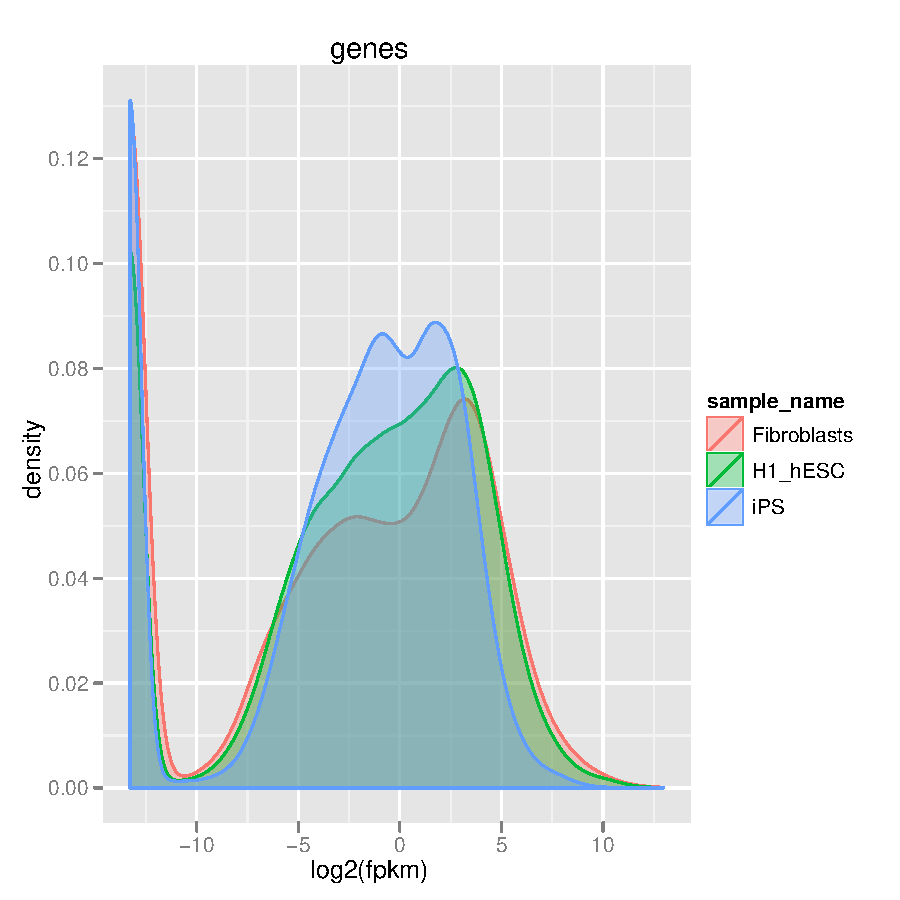
\includegraphics[width=0.4\textwidth]{cummeRbund-manual-global_plots_dens}
	}
	\qquad
	\subfloat[Density plot with replicates=TRUE exposes individual replicate FPKM distributions.]{
	
	
	\includegraphics[width=0.4\textwidth]{cummeRbund-manual-global_plots_dens_rep}}
	\end{center}
\end{figure}

%FPKM distributions - Boxplot
Boxplots can be visualized using the \Rmethod{csBoxplot} method (Figure 2).
\begin{Schunk}
\begin{Sinput}
> b<-csBoxplot(genes(cuff))
> b
> brep<-csBoxplot(genes(cuff),replicates=T)
> brep
\end{Sinput}
\end{Schunk}

\begin{figure}[htp]
	\begin{center}
	\subfloat[Box plot of FPKM distributions for individual conditions.]{
	
	
	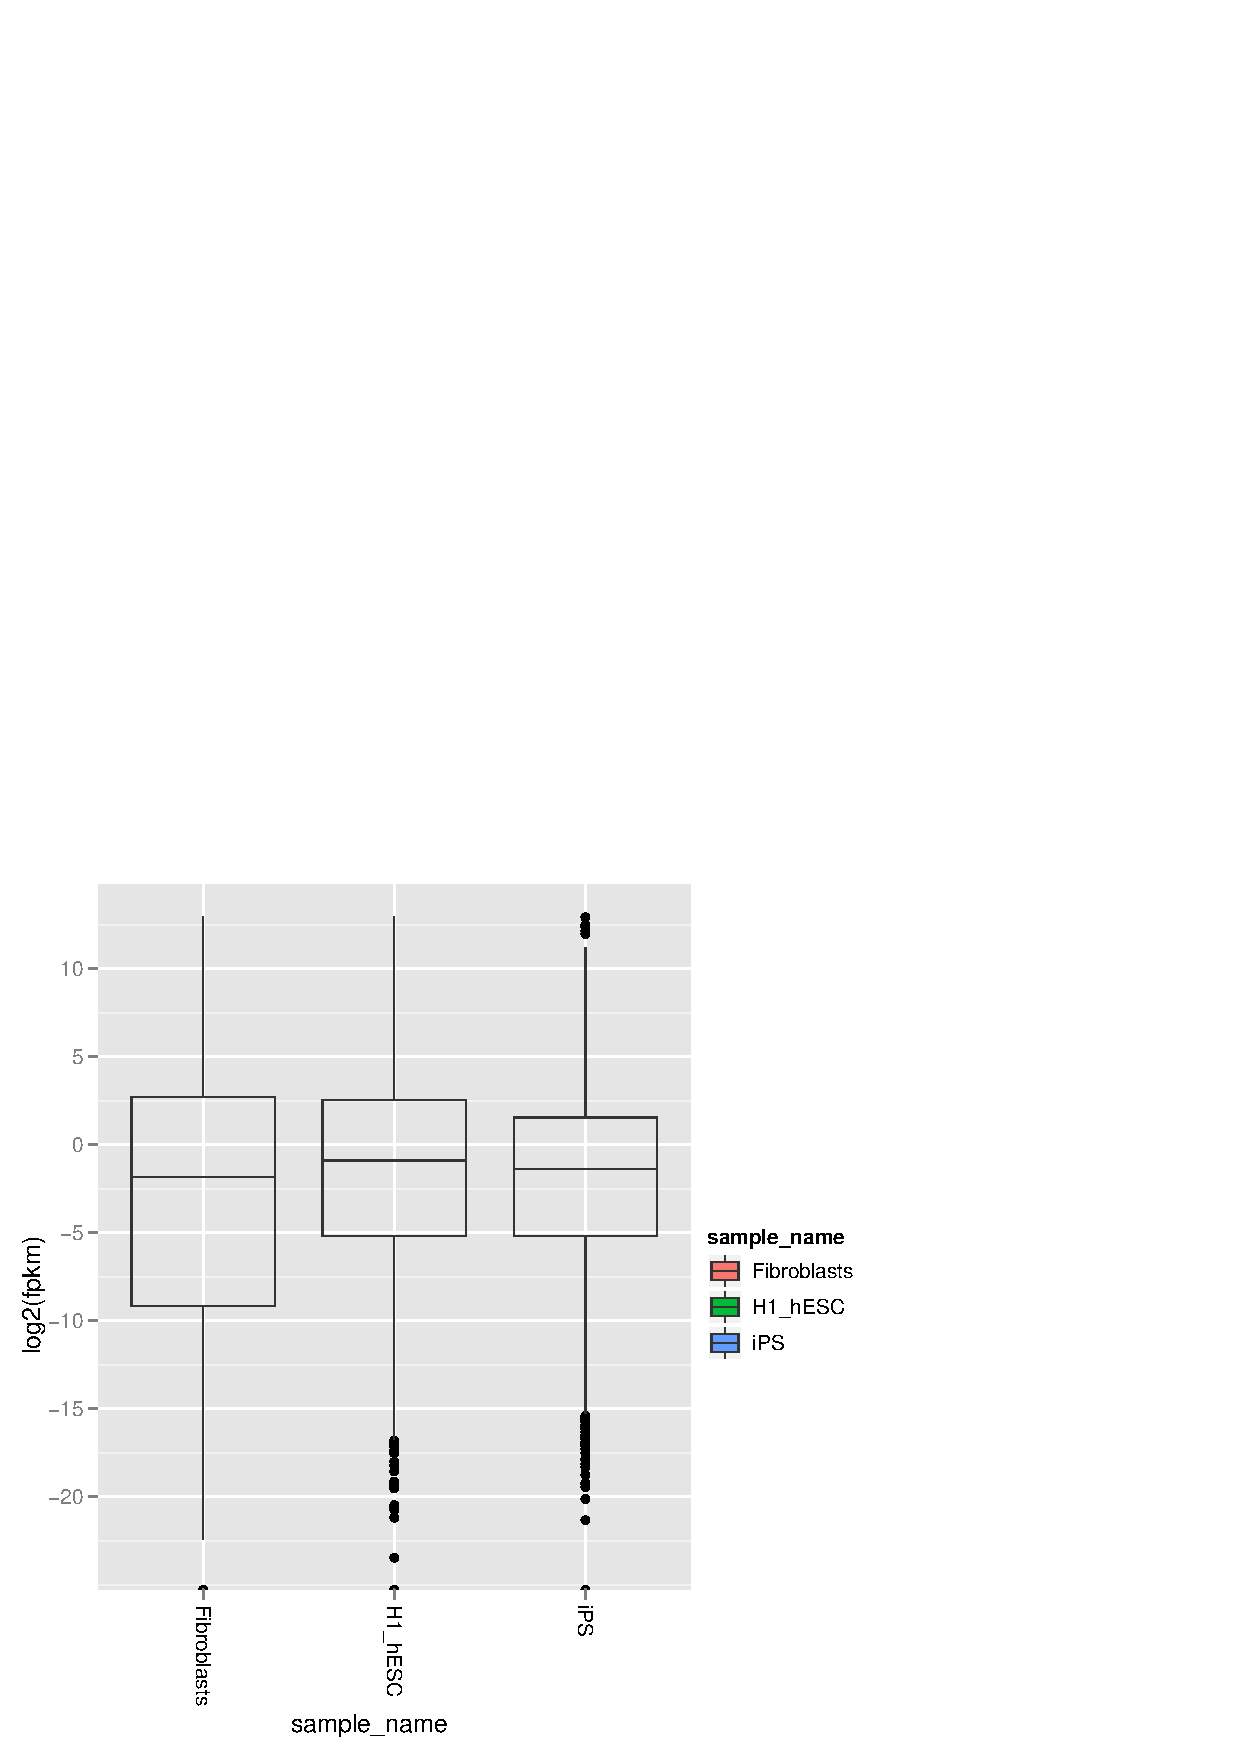
\includegraphics[width=0.4\textwidth]{cummeRbund-manual-global_plots_box}
	}
	\qquad
	\subfloat[Box plot with replicates=TRUE exposes individual replicate FPKM distributions.]{
	
	
	\includegraphics[width=0.4\textwidth]{cummeRbund-manual-global_plots_box_rep}}
	\end{center}
\end{figure}

%Scatterplots
A matrix of pairwise scatterplots can be drawn using the csScatterMatrix()
method.

\begin{Schunk}
\begin{Sinput}
> s<-csScatterMatrix(genes(cuff))
> 
\end{Sinput}
\end{Schunk}

\begin{figure}[htp]
	\begin{center}
	\subfloat[Scatterplots can be useful to identify global changes and trends in gene expression between pairs of conditions.]{
	
	
	\includegraphics[width=0.65\textwidth]{cummeRbund-manual-global_plots_scatter_1}}
	\end{center}
\end{figure}


Individual Pairwise comparisons can be made by using \Rmethod{csScatter}. You
must specify the sample names to use for the $x$ and $y$ axes:
\begin{Schunk}
\begin{Sinput}
> s<-csScatter(genes(cuff),"hESC","Fibroblasts",smooth=T)
> s
\end{Sinput}
\end{Schunk}

\begin{figure}[htp]
	\begin{center}
	\subfloat[Pairwise scatterplots can identify biases in gene expression between
	two particular conditions.]{
	
	
	\includegraphics[width=0.4\textwidth]{cummeRbund-manual-global_plots_scatter_2}}
	\end{center}
\end{figure}

%Dendrograms
\begin{Schunk}
\begin{Sinput}
> dend<-csDendro(genes(cuff))
> dend.rep<-csDendro(genes(cuff),replicates=T)
\end{Sinput}
\end{Schunk}

\begin{figure}[htp]
	\begin{center}
	\subfloat[Dendrogram of JS distances between conditions.]{
	
	
	\includegraphics[width=0.4\textwidth]{cummeRbund-manual-global_plots_dendro}
	}
	\qquad
	\subfloat[Dendrogram with replicates=TRUE can identify outlier replicates.]{
	
	
	\includegraphics[width=0.4\textwidth]{cummeRbund-manual-global_plots_dendro_rep}}
	\end{center}
\end{figure}

%MA plots
MvsA plots can be useful to determine any systematic bias that may be present between conditions. The CuffData method \Rmethod{MAplot()} can be used to examine these intensity vs fold-change plots. You must specify the sample names to use for the pairwise comparison with $x$ and $y$:
\begin{Schunk}
\begin{Sinput}
> m<-MAplot(genes(cuff),"hESC","Fibroblasts")
> m
> mCount<-MAplot(genes(cuff),"hESC","Fibroblasts",useCount=T)
> mCount
\end{Sinput}
\end{Schunk}

\begin{figure}[htp]
	\begin{center}
	\subfloat[MA plots can identify biases across ranges of intensity and fold-change.]{
	
	\includegraphics[width=0.4\textwidth]{cummeRbund-manual-global_plots_MA}}
	
	\qquad
	\subfloat[MA plot drawn on normalized count values instead of FPKM.]{
	
	
	\includegraphics[width=0.4\textwidth]{cummeRbund-manual-global_plots_MA_count}}
	\end{center}
\end{figure}

%Volcano plots
Volcano plots are also available for the \Rclass{CuffData} objects. 

\begin{Schunk}
\begin{Sinput}
> v<-csVolcanoMatrix(genes(cuff))
> v
\end{Sinput}
\end{Schunk}
\begin{figure}[htp]
	\begin{center}
		\subfloat[Volcano plots explore the relationship between fold-change and significance.]{
		
		\includegraphics[width=0.65\textwidth]{cummeRbund-manual-global_plots_volcano_1}}
	\end{center}
\end{figure}

For individual pairwise comparisons, you must specify the comparisons by sample
name.
\begin{Schunk}
\begin{Sinput}
> v<-csVolcano(genes(cuff),"hESC","Fibroblasts")
> v
\end{Sinput}
\end{Schunk}
\begin{figure}[htp]
	\begin{center}
		\subfloat[Volcano plots explore the relationship between fold-change and significance.]{
		
		\includegraphics[width=0.4\textwidth]{cummeRbund-manual-global_plots_volcano_2}}
	\end{center}
\end{figure}

\clearpage

\section{Accessing Data}

\subsection*{Cuffdiff run information}
Run-level information such as run parameters, and sample information can be accessed from a \Rclass{CuffSet} object by using the \Rmethod{runInfo} and \Rmethod{replicates} methods:

\begin{Schunk}
\begin{Sinput}
> runInfo(cuff)
\end{Sinput}
\begin{Soutput}
          param
1      cmd_line
2       version
3  SVN_revision
4 boost_version
5        genome
                                                                                                                                                    value
1 cuffdiff -L iPS,hESC,Fibroblasts -p 6 chr1_snippet.gtf -o iPS_hESC_fibro iPS_rep1.bam,iPS_rep2.bam H1_rep1.bam,H1_rep3.bam NHLF_rep1.bam,NHLF_rep2.bam 
2                                                                                                                                                   1.4.0
3                                                                                                                                                    3285
4                                                                                                                                                  104900
5                                                                                                                                                    hg19
\end{Soutput}
\begin{Sinput}
> replicates(cuff)
\end{Sinput}
\begin{Soutput}
           file sample_name replicate      rep_name total_mass
1  iPS_rep1.bam         iPS         0         iPS_0     173431
2  iPS_rep2.bam         iPS         1         iPS_1     173007
3   H1_rep1.bam        hESC         0        hESC_0     754749
4   H1_rep3.bam        hESC         1        hESC_1     762643
5 NHLF_rep1.bam Fibroblasts         0 Fibroblasts_0     876775
6 NHLF_rep2.bam Fibroblasts         1 Fibroblasts_1    1412130
  norm_mass internal_scale external_scale
1    706934       0.958068       0.584877
2    706934       1.037970       0.584877
3    706934       0.989851       1.513060
4    706934       1.010250       1.513060
5    706934       0.840416       1.223240
6    706934       1.198470       1.223240
\end{Soutput}
\end{Schunk}

\subsection*{Features/Annotation}
Feature-level information can be accessed directly from a \Rclass{CuffData}
object using the \Rmethod{fpkm}, \Rmethod{repFpkm}, \Rmethod{count},
\Rmethod{diffData}, or \Rmethod{annotation} methods:

\begin{Schunk}
\begin{Sinput}
> gene.features<-annotation(genes(cuff))
> head(gene.features)
\end{Sinput}
\begin{Soutput}
      gene_id class_code nearest_ref_id gene_short_name
1 XLOC_000001       <NA>           <NA>            <NA>
2 XLOC_000002       <NA>           <NA>           OR4F5
3 XLOC_000003       <NA>           <NA>            <NA>
4 XLOC_000004       <NA>           <NA>            <NA>
5 XLOC_000005       <NA>           <NA>            <NA>
6 XLOC_000006       <NA>           <NA>          OR4F16
               locus length coverage
1   chr1:11873-29961     NA       NA
2   chr1:69090-70008     NA       NA
3 chr1:321083-321114     NA       NA
4 chr1:321145-321223     NA       NA
5 chr1:322036-328580     NA       NA
6 chr1:367658-368595     NA       NA
\end{Soutput}
\begin{Sinput}
> gene.fpkm<-fpkm(genes(cuff))
> head(gene.fpkm)
\end{Sinput}
\begin{Soutput}
      gene_id sample_name       fpkm    conf_hi conf_lo
1 XLOC_000001 Fibroblasts    16.1506   182.9240 0.00000
2 XLOC_000002 Fibroblasts     0.0000     0.0000 0.00000
3 XLOC_000003 Fibroblasts     0.0000     0.0000 0.00000
4 XLOC_000004 Fibroblasts 14237.7000 78180.9000 0.00000
5 XLOC_000005 Fibroblasts    48.0566    90.6526 5.46055
6 XLOC_000006 Fibroblasts     0.0000     0.0000 0.00000
  quant_status      stdev
1           OK    83.3867
2           OK     0.0000
3           OK     0.0000
4           OK 31971.6000
5           OK    21.2980
6           OK     0.0000
\end{Soutput}
\begin{Sinput}
> gene.repFpkm<-repFpkm(genes(cuff))
> head(gene.repFpkm)
\end{Sinput}
\begin{Soutput}
      gene_id sample_name replicate      rep_name  raw_frags
1 XLOC_000001 Fibroblasts         0 Fibroblasts_0  12.000100
2 XLOC_000002 Fibroblasts         0 Fibroblasts_0   0.000000
3 XLOC_000003 Fibroblasts         0 Fibroblasts_0   0.000000
4 XLOC_000004 Fibroblasts         0 Fibroblasts_0   0.333333
5 XLOC_000005 Fibroblasts         0 Fibroblasts_0 137.100000
6 XLOC_000006 Fibroblasts         0 Fibroblasts_0   0.000000
  internal_scaled_frags external_scaled_frags       fpkm
1             14.278800             11.672900    11.1815
2              0.000000              0.000000     0.0000
3              0.000000              0.000000     0.0000
4              0.396629              0.324245 28475.5000
5            163.134000            133.362000    57.8929
6              0.000000              0.000000     0.0000
  effective_length status
1               NA     OK
2               NA     OK
3               NA     OK
4               NA     OK
5               NA     OK
6               NA     OK
\end{Soutput}
\begin{Sinput}
> gene.counts<-count(genes(cuff))
> head(gene.counts)
\end{Sinput}
\begin{Soutput}
      gene_id sample_name      count    variance uncertainty
1 XLOC_000001 Fibroblasts  20.072500 1.05160e+04 1.77636e-15
2 XLOC_000002 Fibroblasts   0.000000 0.00000e+00 0.00000e+00
3 XLOC_000003 Fibroblasts   0.000000 0.00000e+00 0.00000e+00
4 XLOC_000004 Fibroblasts   0.198315 1.98315e-01 0.00000e+00
5 XLOC_000005 Fibroblasts 131.575000 3.35882e+03 5.68434e-14
6 XLOC_000006 Fibroblasts   0.000000 0.00000e+00 0.00000e+00
   dispersion status
1 1311.870000     OK
2    0.000000     OK
3    0.000000     OK
4    0.198315     OK
5 2161.890000     OK
6    0.000000     OK
\end{Soutput}
\begin{Sinput}
> isoform.fpkm<-fpkm(isoforms(cuff))
> head(isoform.fpkm)
\end{Sinput}
\begin{Soutput}
      isoform_id sample_name        fpkm   conf_hi conf_lo
1 TCONS_00000001 Fibroblasts    10.99630   118.178       0
2 TCONS_00000002 Fibroblasts     0.00000     0.000       0
3 TCONS_00000003 Fibroblasts     5.15434   132.926       0
4 TCONS_00000004 Fibroblasts     0.00000     0.000       0
5 TCONS_00000005 Fibroblasts     0.00000     0.000       0
6 TCONS_00000006 Fibroblasts 14237.70000 78180.900       0
  quant_status       stdev
1           OK    53.59085
2           OK     0.00000
3           OK    63.88583
4           OK     0.00000
5           OK     0.00000
6           OK 31971.60000
\end{Soutput}
\begin{Sinput}
> gene.diff<-diffData(genes(cuff))
> head(gene.diff)
\end{Sinput}
\begin{Soutput}
      gene_id sample_1 sample_2 status   value_1     value_2
1 XLOC_000001      iPS     hESC NOTEST  20.21750 3.47386e-01
2 XLOC_000002      iPS     hESC NOTEST   0.00000 0.00000e+00
3 XLOC_000003      iPS     hESC NOTEST   0.00000 0.00000e+00
4 XLOC_000004      iPS     hESC     OK   0.00000 6.97259e+05
5 XLOC_000005      iPS     hESC     OK 355.82300 6.96704e+02
6 XLOC_000006      iPS     hESC NOTEST   1.51396 0.00000e+00
  log2_fold_change     test_stat    p_value    q_value
1     -5.86292e+00   7.13525e-01 0.47552100 1.00000000
2      0.00000e+00   0.00000e+00 1.00000000 1.00000000
3      0.00000e+00   0.00000e+00 1.00000000 1.00000000
4     1.79769e+308  1.79769e+308 0.00857693 0.02109120
5      9.69385e-01  -2.98373e+00 0.00284757 0.00840284
6    -1.79769e+308 -1.79769e+308 0.24382400 1.00000000
  significant
1          no
2          no
3          no
4         yes
5         yes
6          no
\end{Soutput}
\end{Schunk}

\subsection*{Condition and feature names}
Vectors of sample names and feature names are available by using the \Rmethod{samples} and \Rmethod{featureNames} methods:

\begin{Schunk}
\begin{Sinput}
> sample.names<-samples(genes(cuff))
> head(sample.names)
\end{Sinput}
\begin{Soutput}
[1] "iPS"         "hESC"        "Fibroblasts"
\end{Soutput}
\begin{Sinput}
> gene.featurenames<-featureNames(genes(cuff))
> head(gene.featurenames)
\end{Sinput}
\begin{Soutput}
[1] "XLOC_000001" "XLOC_000002" "XLOC_000003" "XLOC_000004"
[5] "XLOC_000005" "XLOC_000006"
\end{Soutput}
\end{Schunk}

\subsection*{Convenience functions}
To facilitate Bioconductor-like operations, an 'FPKM-matrix' can be returned easily using the \Rmethod{fpkmMatrix} method:
\begin{Schunk}
\begin{Sinput}
> gene.matrix<-fpkmMatrix(genes(cuff))
> head(gene.matrix)
\end{Sinput}
\begin{Soutput}
                  iPS        hESC Fibroblasts
XLOC_000001  20.21750 3.47386e-01     16.1506
XLOC_000002   0.00000 0.00000e+00      0.0000
XLOC_000003   0.00000 0.00000e+00      0.0000
XLOC_000004   0.00000 6.97259e+05  14237.7000
XLOC_000005 355.82300 6.96704e+02     48.0566
XLOC_000006   1.51396 0.00000e+00      0.0000
\end{Soutput}
\end{Schunk}

A matrix of replicate FPKM values can be retrieved by using \Rmethod{repFpkmMatrix}
\begin{Schunk}
\begin{Sinput}
> gene.rep.matrix<-repFpkmMatrix(genes(cuff))
> head(gene.rep.matrix)
\end{Sinput}
\begin{Soutput}
               iPS_0     iPS_1      hESC_0      hESC_1
XLOC_000001  17.2049  22.92880       0.000 6.21918e-01
XLOC_000002   0.0000   0.00000       0.000 0.00000e+00
XLOC_000003   0.0000   0.00000       0.000 0.00000e+00
XLOC_000004   0.0000   0.00000 1377990.000 8.35811e+05
XLOC_000005 319.0300 390.45500     687.563 7.21983e+02
XLOC_000006   0.0000   3.02791       0.000 0.00000e+00
            Fibroblasts_0 Fibroblasts_1
XLOC_000001       11.1815       20.6009
XLOC_000002        0.0000        0.0000
XLOC_000003        0.0000        0.0000
XLOC_000004    28475.5000        0.0000
XLOC_000005       57.8929       38.0084
XLOC_000006        0.0000        0.0000
\end{Soutput}
\end{Schunk}

Similarly, a matrix of normalized counts can be generated by using \Rmethod{countMatrix}
\begin{Schunk}
\begin{Sinput}
> gene.count.matrix<-countMatrix(genes(cuff))
> head(gene.count.matrix)
\end{Sinput}
\begin{Soutput}
                   iPS        hESC Fibroblasts
XLOC_000001  11.440900    0.494996   20.072500
XLOC_000002   0.000000    0.000000    0.000000
XLOC_000003   0.000000    0.000000    0.000000
XLOC_000004   0.000000    5.680560    0.198315
XLOC_000005 486.456000 2495.560000  131.575000
XLOC_000006   0.481711    0.000000    0.000000
\end{Soutput}
\end{Schunk}

\subsection{Writing your own SQL accessors}
Since the cuffData.db is a SQLite database backend, if you are familiar with SQL and/or RSQLite query construction, you can simply design your own SQL queries to access the data that you are after. 

\begin{figure}[h]
\centering

\includegraphics[angle=90, height=\textheight]{cuffData_schema.pdf}

\end{figure}

\clearpage 

\section{Creating Gene Sets}
Gene Sets (stored in a \Rclass{CuffGeneSet} object) can be created using the \Rmethod{getGenes} method on a CuffSet object.
You must first create a vector of 'gene\_id' or 'gene\_short\_name' values to identify the genes you wish to select:

\begin{Schunk}
\begin{Sinput}
> data(sampleData)
> myGeneIds<-sampleIDs
> myGeneIds
\end{Sinput}
\begin{Soutput}
 [1] "XLOC_001363" "XLOC_001297" "XLOC_001339" "XLOC_000132"
 [5] "XLOC_001265" "XLOC_000151" "XLOC_001359" "XLOC_000069"
 [9] "XLOC_000170" "XLOC_000105" "XLOC_001262" "XLOC_001348"
[13] "XLOC_001411" "XLOC_001369" "XLOC_000158" "XLOC_001370"
[17] "XLOC_001263" "XLOC_000115" "XLOC_000089" "XLOC_001240"
\end{Soutput}
\begin{Sinput}
> myGenes<-getGenes(cuff,myGeneIds)
> myGenes
\end{Sinput}
\begin{Soutput}
CuffGeneSet instance for  20  genes
 
Slots:
	 annotation
	 fpkm
	 repFpkm
	 diff
	 count
	 isoforms	 CuffFeatureSet instance of size 45 
	 TSS		 CuffFeatureSet instance of size 23 
	 CDS		 CuffFeatureSet instance of size 36 
	 promoters		 CuffFeatureSet instance of size 20 
	 splicing		 CuffFeatureSet instance of size 23 
	 relCDS		 CuffFeatureSet instance of size 20 
\end{Soutput}
\end{Schunk}
The same \Rmethod{fpkm}, \Rmethod{repFpkm}, \Rmethod{count}, \Rmethod{annotation}, \Rmethod{diffData}, \Rmethod{samples}, and \Rmethod{featureNames} methods are available for instances of the \Rmethod{CuffGeneSet} class, but additional accessor methods are available for the \Rmethod{promoters}, \Rmethod{relCDS}, and \Rmethod{splicing} slot data as well.

\begin{Schunk}
\begin{Sinput}
> #FPKM values for genes in gene set
> head(fpkm(myGenes))
\end{Sinput}
\begin{Soutput}
      gene_id sample_name        fpkm     conf_hi  conf_lo
1 XLOC_000069 Fibroblasts 2.05083e-01 8.94501e-01    0.000
2 XLOC_000069        hESC 1.77686e+02 2.15888e+02  139.484
3 XLOC_000069         iPS 1.90000e+01 3.88149e+01    0.000
4 XLOC_000089 Fibroblasts 1.39701e+04 2.19187e+04 6021.450
5 XLOC_000089        hESC 7.18339e+03 7.92296e+03 6443.810
6 XLOC_000089         iPS 1.41690e+03 1.96558e+03  868.215
  quant_status       stdev
1           OK    0.344709
2           OK   19.101000
3           OK    9.907450
4           OK 3974.300000
5           OK  369.785000
6           OK  274.340000
\end{Soutput}
\begin{Sinput}
> #Isoform-level FPKMs for gene set
> head(fpkm(isoforms(myGenes)))
\end{Sinput}
\begin{Soutput}
      isoform_id sample_name       fpkm    conf_hi   conf_lo
1 TCONS_00000179 Fibroblasts   0.205083   0.894501   0.00000
2 TCONS_00000179        hESC  20.360900  33.840500   6.88119
3 TCONS_00000179         iPS   7.694340  16.356900   0.00000
4 TCONS_00000180 Fibroblasts   0.000000   0.000000   0.00000
5 TCONS_00000180        hESC 157.325000 198.673000 115.97800
6 TCONS_00000180         iPS  11.305600  27.105700   0.00000
  quant_status     stdev
1           OK  0.344709
2           OK  6.739800
3           OK  4.331280
4           OK  0.000000
5           OK 20.674000
6           OK  7.900050
\end{Soutput}
\begin{Sinput}
> #Replicate FPKMs for TSS groups within gene set
> head(repFpkm(TSS(myGenes)))
\end{Sinput}
\begin{Soutput}
  TSS_group_id sample_name replicate      rep_name raw_frags
1       TSS128         iPS         0         iPS_0     987.0
2       TSS128         iPS         1         iPS_1    1065.0
3       TSS128        hESC         1        hESC_1   13196.0
4       TSS128        hESC         0        hESC_0   13588.0
5       TSS128 Fibroblasts         1 Fibroblasts_1   18899.5
6       TSS128 Fibroblasts         0 Fibroblasts_0   22201.0
  internal_scaled_frags external_scaled_frags     fpkm
1               1030.20               1761.39  1412.22
2               1026.04               1754.29  1404.74
3              13062.10               8632.91  7131.86
4              13727.30               9072.58  7500.15
5              15769.70              12891.80 10368.60
6              26416.70              21595.70 17372.90
  effective_length status
1               NA     OK
2               NA     OK
3               NA     OK
4               NA     OK
5               NA     OK
6               NA     OK
\end{Soutput}
\begin{Sinput}
> 
\end{Sinput}
\end{Schunk}

As of \Rpackage{cummeRbund} $v2.0$ \Rclass{CuffGeneSet} classes can be created from any type of identifier ('gene\_id','isoform\_id','TSS\_group\_id', or 'CDS\_id'). When you pass a list of identifiers that are not gene\_id to \Rmethod{getGenes()}, the function attempts to lookup the parent gene\_id for each feature and returns \emph{all} relevant
information for the given genes and all of their sub-features (not just the sub-features passed to \Rmethod{getGenes()}).  If you are interested in just retrieving information for a given set of features, please use the new \Rmethod{getFeatures()} method described later.

\subsection{Geneset level plots}
There are several plotting functions available for gene-set-level visualization:

The \Rmethod{csHeatmap()} function is a plotting wrapper that takes as input either a CuffGeneSet or a CuffFeatureSet object (essentially a collection of genes and/or features) and produces a heatmap of FPKM expression values.  The 'cluster' argument can be used to re-order either 'row', 'column', or 'both' dimensions of this matrix.
By default, the Jensen-Shannon distance is used as the clustering metric, however, any function that produces a \Rclass{dist} object can be passed to the 'cluster' argument as well.

\begin{Schunk}
\begin{Sinput}
> h<-csHeatmap(myGenes,cluster='both')
> h
> h.rep<-csHeatmap(myGenes,cluster='both',replicates=T)
> h.rep
\end{Sinput}
\end{Schunk}

\begin{figure}[htp]
	\begin{center}
	\subfloat[Heatmaps provide a convenient way to visualize the expression of entire gene sets at once.]{
	
	\includegraphics[width=0.4\textwidth]{cummeRbund-manual-geneset_plots_heatmap}}
	
	\qquad
	\subfloat[Same heatmap, with replicates=T can help to visualize variance between replicates.]{
	
	\includegraphics[width=0.4\textwidth]{cummeRbund-manual-geneset_plots_heatmap_rep}}
	\end{center}
\end{figure}

If you prefer barplots over heatmaps for genesets (although this is not necessarily recommended for large gene sets). You can use the \Rmethod{expressionBarplot()} method on a \Rclass{CuffFeatureSet} or a \Rclass{CuffGeneSet} object.
\begin{Schunk}
\begin{Sinput}
> b<-expressionBarplot(myGenes)
> b
\end{Sinput}
\end{Schunk}
\begin{figure}[htp]
	\begin{center}
		\subfloat[A (somewhat crowded) barplot for all genes in a CuffGeneSet object.]{
		
		\includegraphics[width=0.9\textwidth]{cummeRbund-manual-geneset_plots_barplot}}
	\end{center}
\end{figure}

The \Rmethod{csScatter()} method can be used to produce scatter plot comparisons between any two conditions.
\begin{Schunk}
\begin{Sinput}
> s<-csScatter(myGenes,"Fibroblasts","hESC",smooth=T)
> s
\end{Sinput}
\end{Schunk}

\begin{figure}[htp]
	\begin{center}
		\subfloat[Scatterplot showing relationship between two conditions for genes in a CuffGeneSet.]{
		
		\includegraphics[width=0.4\textwidth]{cummeRbund-manual-geneset_plots_scatter}}
	\end{center}
\end{figure}


The volcano plot is a useful visualization to compare fold change between any two conditions and significance (-log P-values).
\begin{Schunk}
\begin{Sinput}
> v<-csVolcano(myGenes,"Fibroblasts","hESC")
> v
\end{Sinput}
\end{Schunk}

\begin{figure}[htp]
	\begin{center}
		\subfloat[Fold-change vs significance for genes in a CuffGeneSet object.]{
		
		\includegraphics[width=0.4\textwidth]{cummeRbund-manual-geneset_plots_volcano}}
	\end{center}
\end{figure}


Similar plots can be made for all sub-level features of a \Rclass{CuffGeneSet} class by specifying which slot you would like to plot (eg. \Rfunarg{isoforms(myGenes)},\Rfunarg{TSS(myGenes)},\Rfunarg{CDS(myGenes)}).

\begin{Schunk}
\begin{Sinput}
> ih<-csHeatmap(isoforms(myGenes),cluster='both',labRow=F)
> ih
> th<-csHeatmap(TSS(myGenes),cluster='both',labRow=F)
> th
\end{Sinput}
\end{Schunk}
\begin{figure}[htp]
	\begin{center}
		\subfloat[A heatmap of isoform-level FPKM values for all genes in a CuffGeneSet object.]{
		
		\includegraphics[width=0.4\textwidth]{cummeRbund-manual-geneset_plots_isoform_heatmap}}
		\qquad
		\subfloat[A heatmap of TSS-level FPKM values for all genes in a CuffGeneSet object.]{
		
		\includegraphics[width=0.4\textwidth]{cummeRbund-manual-geneset_plots_TSS_heatmap}}
	
	\end{center}
\end{figure}

Dendrograms can provide insight into the relationships between conditions for various genesets (e.g. significant genes used to draw relationships between conditions). As of v1.1.3 the method \Rmethod{csDendro()}
can be used to plot a dendrogram based on Jensen-Shannon distances between conditions for a given \Rclass{CuffFeatureSet} or \Rclass{CuffGeneSet}.
\begin{Schunk}
\begin{Sinput}
> den<-csDendro(myGenes)
\end{Sinput}
\end{Schunk}
\begin{figure}[htp]
	\begin{center}
		\subfloat[A dendrogram of the relationship between conditions based on the expression of genes in a CuffGeneSet.]{
		
		\includegraphics[width=0.4\textwidth]{cummeRbund-manual-geneset_plots_dendro}}
	
	\end{center}
\end{figure}

\clearpage

\section{Individual Genes}
An individual CuffGene object can be created by using the \Rfunction{getGene()} function for a given 'gene\_id' or 'gene\_short\_name'. As of cummeRbund $\ge v2.0$ you can also use isoform\_id, tss\_group\_id, or
cds\_id values to retrieve the corresponding parent gene object.

\begin{Schunk}
\begin{Sinput}
> myGeneId<-"PINK1"
> myGene<-getGene(cuff,myGeneId)
> myGene
\end{Sinput}
\begin{Soutput}
CuffGene instance for gene XLOC_000172 
Short name:	 PINK1 
Slots:
	 annotation
	 features
	 fpkm
	 repFpkm
	 diff
	 count
	 isoforms	 CuffFeature instance of size 2 
	 TSS		 CuffFeature instance of size 2 
	 CDS		 CuffFeature instance of size 2 
\end{Soutput}
\begin{Sinput}
> head(fpkm(myGene))
\end{Sinput}
\begin{Soutput}
      gene_id sample_name     fpkm  conf_hi  conf_lo
1 XLOC_000172 Fibroblasts 3045.930 4529.840 1562.020
2 XLOC_000172        hESC  441.939  523.916  359.961
3 XLOC_000172         iPS  640.208  914.562  365.853
  quant_status
1           OK
2           OK
3           OK
\end{Soutput}
\begin{Sinput}
> head(fpkm(isoforms(myGene)))
\end{Sinput}
\begin{Soutput}
      isoform_id sample_name     fpkm  conf_hi   conf_lo
1 TCONS_00000480 Fibroblasts 2213.850 3284.980 1142.7100
2 TCONS_00000480        hESC  326.979  388.108  265.8500
3 TCONS_00000480         iPS  640.208  914.562  365.8530
4 TCONS_00000481 Fibroblasts  832.083 1760.820    0.0000
5 TCONS_00000481        hESC  114.960  166.530   63.3891
6 TCONS_00000481         iPS    0.000    0.000    0.0000
  quant_status
1           OK
2           OK
3           OK
4           OK
5           OK
6           OK
\end{Soutput}
\end{Schunk}

\subsection{Gene-level plots}
\begin{Schunk}
\begin{Sinput}
> gl<-expressionPlot(myGene)
> gl
> gl.rep<-expressionPlot(myGene,replicates=TRUE)
> gl.rep
> gl.iso.rep<-expressionPlot(isoforms(myGene),replicates=T)
> gl.iso.rep
> gl.cds.rep<-expressionPlot(CDS(myGene),replicates=T)
> gl.cds.rep
\end{Sinput}
\end{Schunk}

\begin{figure}[htp]
	\begin{center}
	\subfloat[Expression plot of a single gene.]{
	
	
	\includegraphics[width=0.4\textwidth]{cummeRbund-manual-gene_plots_line}
	}
	\qquad
	\subfloat[Expression plot of a single gene with replicate FPKMs exposed.]{
	
	
	\includegraphics[width=0.4\textwidth]{cummeRbund-manual-gene_plots_replicate_line}}
	\qquad
	\subfloat[Expression plot of all isoforms of a single gene with replicate FPKMs exposed.]{
	
	
	\includegraphics[width=0.4\textwidth]{cummeRbund-manual-gene_plots_iso_replicate_line}}
	\qquad
	\subfloat[Expression plot of all CDS for a single gene with replicate FPKMs exposed.]{
	
	
	\includegraphics[width=0.4\textwidth]{cummeRbund-manual-gene_plots_cds_replicate_line}}
	\end{center}
\end{figure}


\begin{Schunk}
\begin{Sinput}
> gb<-expressionBarplot(myGene)
> gb
> gb.rep<-expressionBarplot(myGene,replicates=T)
> gb.rep
\end{Sinput}
\end{Schunk}

\begin{figure}[htp]
	\begin{center}
	\subfloat[Expression Barplot of a single gene.]{
	
	
	\includegraphics[width=0.4\textwidth]{cummeRbund-manual-gene_plots_bar}
	}
	\qquad
	\subfloat[Expression Barplot of a single gene with replicate FPKMs exposed.]{
	

	
	\includegraphics[width=0.4\textwidth]{cummeRbund-manual-gene_plots_bar_rep}}
	\end{center}
\end{figure}


\begin{Schunk}
\begin{Sinput}
> igb<-expressionBarplot(isoforms(myGene),replicates=T)
> igb
\end{Sinput}
\end{Schunk}

\begin{figure}[htp]
	\begin{center}
	\subfloat[Expression Barplot of all isoforms single gene with replicates exposed.]{
	
	\includegraphics[width=0.4\textwidth]{cummeRbund-manual-gene_plots_bar_isoforms}
	}
	
	\end{center}
\end{figure}

\clearpage

\subsubsection{Gene Feature plots}
If you included both the genome build and gtfFile in your call to \Rmethod{readCufflinks()} then you will be able to access some of the transcript-structure level features that are now being integrated into cummeRbund. For now, these features are extended only to the single gene, \Rclass{CuffGene} objects.

Feature data are loaded into the \'features\' table of the cuffData.db database. When a \Rclass{CuffGene} object is created using \Rmethod{getGene()}, all relative features are selected from this table and a \'features\' slot is added to the resulting object.

\begin{Schunk}
\begin{Sinput}
> head(features(myGene))
\end{Sinput}
\begin{Soutput}
  seqnames    start      end width strand source type score
1     chr1 20959948 20960428   481      + coding exon    NA
2     chr1 20964335 20964622   288      + coding exon    NA
3     chr1 20966385 20966485   101      + coding exon    NA
4     chr1 20970983 20971165   183      + coding exon    NA
5     chr1 20972053 20972216   164      + coding exon    NA
6     chr1 20974998 20975125   128      + coding exon    NA
  phase class_code exon_number     gene_id gene_name nearest_ref
1    NA          =           1 XLOC_000172     PINK1  uc001bdm.2
2    NA          =           2 XLOC_000172     PINK1  uc001bdm.2
3    NA          =           3 XLOC_000172     PINK1  uc001bdm.2
4    NA          =           4 XLOC_000172     PINK1  uc001bdm.2
5    NA          =           5 XLOC_000172     PINK1  uc001bdm.2
6    NA          =           6 XLOC_000172     PINK1  uc001bdm.2
         oId CDS_id     isoform_id TSS_group_id
1 uc001bdm.2   P364 TCONS_00000480       TSS264
2 uc001bdm.2   P364 TCONS_00000480       TSS264
3 uc001bdm.2   P364 TCONS_00000480       TSS264
4 uc001bdm.2   P364 TCONS_00000480       TSS264
5 uc001bdm.2   P364 TCONS_00000480       TSS264
6 uc001bdm.2   P364 TCONS_00000480       TSS264
\end{Soutput}
\end{Schunk}

The \Rpackage{Gviz} package can be used to display features in a 'track'-like format. In particular, the \Rclass{GeneRegionTrack} class creates a mechanism by which we can start to visualize transcript-level structures in their genomic context. \Rpackage{cummeRbund} implements the \Rmethod{makeGeneRegionTrack()} method to quickly create a \Rclass{GeneRegionTrack} from the gene features.

\begin{Schunk}
\begin{Sinput}
> genetrack<-makeGeneRegionTrack(myGene)
> plotTracks(genetrack)
\end{Sinput}
\end{Schunk}
\includegraphics{graphics/cummeRbund-manual-features_2}

We can then use some of the additional features from the \Rpackage{Gviz} package
to add additional tracks from an external data source.

\begin{Schunk}
\begin{Sinput}
> trackList<-list()
> myStart<-min(features(myGene)$start)
> myEnd<-max(features(myGene)$end)
> myChr<-unique(features(myGene)$seqnames)
> genome<-'hg19'
> ideoTrack <- IdeogramTrack(genome = genome, chromosome = myChr)
> trackList<-c(trackList,ideoTrack)
> axtrack<-GenomeAxisTrack()
> trackList<-c(trackList,axtrack)
> genetrack<-makeGeneRegionTrack(myGene)
> genetrack
\end{Sinput}
\begin{Soutput}
GeneRegionTrack 'CuffDiff'
| genome: hg19
| active chromosome: chr1
| annotation features: 12
\end{Soutput}
\begin{Sinput}
> trackList<-c(trackList,genetrack)
> biomTrack<-BiomartGeneRegionTrack(genome=genome,chromosome=as.character(myChr),
+ 		start=myStart,end=myEnd,name="ENSEMBL",showId=T)
> trackList<-c(trackList,biomTrack)
> conservation <- UcscTrack(genome = genome, chromosome = myChr,
+ 		track = "Conservation", table = "phyloP46wayPlacental",
+ 		from = myStart-2000, to = myEnd+2000, trackType = "DataTrack",
+ 		start = "start", end = "end", data = "score",
+ 		type = "hist", window = "auto", col.histogram = "darkblue",
+ 		fill.histogram = "darkblue", ylim = c(-3.7, 4),
+ 		name = "Conservation")
> trackList<-c(trackList,conservation)
> plotTracks(trackList,from=myStart-2000,to=myEnd+2000)
> 
\end{Sinput}
\end{Schunk}
\includegraphics{graphics/cummeRbund-manual-features_3}

\clearpage

\section{Data Exploration}
The cummeRbund package is more than just a visualization tool as well.  We are working to implement several different means of data exploration from gene and condition clustering, finding features with similar expression profiles, as well as incorporating Gene Ontology analysis.

\subsection{Overview of significant features}
The \Rmethod{sigMatrix()} function can provide you with a ``quick--and--dirty''
view of the number of significant features of a particular type, and at a given alpha ($0.05$ by default). For example:

\begin{Schunk}
\begin{Sinput}
> mySigMat<-sigMatrix(cuff,level='genes',alpha=0.05)
> 
\end{Sinput}
\end{Schunk}

\begin{figure}[htp]
	\begin{center}
	\subfloat[Significant features overview matrix. This plot describes the number of significant genes at a 5\%FDR for each pairwise interaction tested.]{
	
	\includegraphics[width=0.6\textwidth]{cummeRbund-manual-sig_mat_plot_1}}
	
	\end{center}
\end{figure}

\subsection{Creating gene sets from significantly regulated genes}
One of the primary roles of a differential expression analysis is to conduct significance tests on each feature (genes, isoforms, TSS, and CDS) for appropriate pairwise comparisons of conditions. The results of these tests (after multiple testing correction of course) can be used to determine which genes are differentially regulated. 
\Rpackage{cummeRbund} makes accessing the results of these significance tests simple via \Rmethod{getSig()}. This function takes a CuffSet object and will scan at various feature levels ('genes' by default) to produce a \Rclass{vector} of feature IDs.
By default \Rmethod{getSig()} outputs a vector of tracking IDs corresponding to all \emph{genes} that reject the null hypothesis in any condition tested. The default feature type can be changed by adjusting the 'level' argument to \Rmethod{getSig()}. In addition, a alpha value can be provided on which to filter the resulting list
(the default is $0.05$ to match the default of cuffdiff). 

\begin{Schunk}
\begin{Sinput}
> mySigGeneIds<-getSig(cuff,alpha=0.05,level='genes')
> head(mySigGeneIds)
\end{Sinput}
\begin{Soutput}
[1] "XLOC_000004" "XLOC_000005" "XLOC_000008" "XLOC_000009"
[5] "XLOC_000011" "XLOC_000013"
\end{Soutput}
\begin{Sinput}
> length(mySigGeneIds)
\end{Sinput}
\begin{Soutput}
[1] 207
\end{Soutput}
\end{Schunk}
By default \Rmethod{getSig()} outputs a vector of tracking IDs corresponding to all \emph{genes} that reject the null hypothesis in any condition tested. The default feature type can be changed by adjusting the 'level' argument to \Rmethod{getSig()}. In addition, a alpha value can be provided on which to filter the resulting list
(the default is $0.05$ to match the default of cuffdiff). Significance results for specific pairwise comparisons can be retrieved as well by specifying the two conditions as 'x' and 'y'. In this case, p-values are adjusted to reduce the impact of multiple-testing correction when only one set of tests is being conducted.

\begin{Schunk}
\begin{Sinput}
> hESC_vs_iPS.sigIsoformIds<-getSig(cuff,x='hESC',y='iPS',alpha=0.05,level='isoforms')
> head(hESC_vs_iPS.sigIsoformIds)
\end{Sinput}
\begin{Soutput}
[1] "TCONS_00000006" "TCONS_00000013" "TCONS_00000015"
[4] "TCONS_00000018" "TCONS_00000034" "TCONS_00000041"
\end{Soutput}
\begin{Sinput}
> length(hESC_vs_iPS.sigIsoformIds)
\end{Sinput}
\begin{Soutput}
[1] 118
\end{Soutput}
\end{Schunk}
The values returned for each level of this list can be used as an argument to getGenes, to create a \Rclass{CuffGeneSet} object of significantly regulated genes (or features).

\begin{Schunk}
\begin{Sinput}
> mySigGenes<-getGenes(cuff,mySigGeneIds)
> mySigGenes
\end{Sinput}
\begin{Soutput}
CuffGeneSet instance for  207  genes
 
Slots:
	 annotation
	 fpkm
	 repFpkm
	 diff
	 count
	 isoforms	 CuffFeatureSet instance of size 717 
	 TSS		 CuffFeatureSet instance of size 399 
	 CDS		 CuffFeatureSet instance of size 577 
	 promoters		 CuffFeatureSet instance of size 207 
	 splicing		 CuffFeatureSet instance of size 399 
	 relCDS		 CuffFeatureSet instance of size 207 
\end{Soutput}
\begin{Sinput}
> 
\end{Sinput}
\end{Schunk}
Alternatively, you can use the \Rmethod{getSigTable()} method to return a full test-table of 'significant features' x 'pairwise tests' for all comparisons. Only features in which the null hypothesis can be rejected in at least one test are reported.

\begin{Schunk}
\begin{Sinput}
> mySigTable<-getSigTable(cuff,alpha=0.01,level='genes')
> head(mySigTable,20)
\end{Sinput}
\begin{Soutput}
            hESCvsFibroblasts iPSvsFibroblasts iPSvshESC
XLOC_000005                 1                1         1
XLOC_000008                 0                1         1
XLOC_000009                 1                1         1
XLOC_000011                 0                1         1
XLOC_000013                 0                1         0
XLOC_000014                 1               NA         0
XLOC_000016                 0                0         1
XLOC_000017                 0                1         0
XLOC_000018                 1                1         0
XLOC_000019                 0                1         1
XLOC_000025                 1               NA         1
XLOC_000026                 1                1         0
XLOC_000027                 0                1         1
XLOC_000029                 1                1         0
XLOC_000032                 1               NA         0
XLOC_000034                 1                0         1
XLOC_000036                 0                1         1
XLOC_000044                 1               NA         1
XLOC_000047                 1                1         1
XLOC_000048                 1                1         0
\end{Soutput}
\end{Schunk}

\subsection{Exploring the relationships between conditions}

\subsubsection{Distance matrix}
Similarities between conditions and/or replicates can
provide useful insight into the relationship between various groupings of
conditions and can aid in identifying outlier replicates that do not behave as
expected. cummeRbund provides the \Rmethod{csDistHeat()} method to visualize the
pairwise similarities between conditions:

\begin{Schunk}
\begin{Sinput}
> myDistHeat<-csDistHeat(genes(cuff))
> 
\end{Sinput}
\end{Schunk}

\begin{figure}[htp]
	\begin{center}
	\subfloat[JS distance heatmap between conditions across all gene features.]{
	
	\includegraphics[width=0.6\textwidth]{cummeRbund-manual-dist_heat_plot_1}}
	
	\end{center}
\end{figure}

Again with the \Rfunarg{replicates} argument, distances between individual
replicates can be presented.

\begin{Schunk}
\begin{Sinput}
> myRepDistHeat<-csDistHeat(genes(cuff),replicates=T)
> 
\end{Sinput}
\end{Schunk}

\begin{figure}[htp]
	\begin{center}
	\subfloat[JS distance heatmap between replicate samples across all gene
	features.]{
	
	\includegraphics[width=0.6\textwidth]{cummeRbund-manual-dist_heat_plot_2}}
	
	\end{center}
\end{figure}

This method can be used to explore similarities between conditions for all
features, or just those features contained within a \Rclass{CuffGeneSet} class. 
Additionally, the \Rfunarg{samples.not.genes=F} argument will display distances
between individual genes or features across conditions.

\subsubsection{Dimensionality reduction}
Dimensionality reduction is an informative approach for clustering and exploring
the relationships between conditions.  It can be useful for feature selection as
well as identifying the sources of variability within your data.  To this end,
we have applied two different dimensionality reduction strategies in
\Rpackage{cummeRbund}: principal component analysis (PCA) and multi-dimensional
scaling (MDS). We provide the two wrapper methods, \Rmethod{PCAplot} and
\Rmethod{MDSplot}

\begin{Schunk}
\begin{Sinput}
> genes.PCA<-PCAplot(genes(cuff),"PC1","PC2")
> genes.MDS<-MDSplot(genes(cuff))
> genes.PCA.rep<-PCAplot(genes(cuff),"PC1","PC2",replicates=T)
> genes.MDS.rep<-MDSplot(genes(cuff),replicates=T)
\end{Sinput}
\end{Schunk}

\begin{figure}[htp]
	\begin{center}
	\subfloat[PCA plot for gene-level features]{
	
	
	\includegraphics[width=0.4\textwidth]{cummeRbund-manual-gene_PCA}
	}
	\qquad
	\subfloat[MDS plot for gene-level features]{
	
	
	\includegraphics[width=0.4\textwidth]{cummeRbund-manual-gene_MDS}}
	\qquad
	\subfloat[Individual replicate level PCA plot for gene-level features]{
	
	
	\includegraphics[width=0.4\textwidth]{cummeRbund-manual-gene_PCA_rep}}
	\qquad
	\subfloat[Individual replicate level MDS plot for gene-level features]{
	
	
	\includegraphics[width=0.4\textwidth]{cummeRbund-manual-gene_MDS_rep}}
	\end{center}
\end{figure}

\clearpage

\subsection{Partitioning}
K-means clustering is a useful tool that can be helpful in identifying clusters of genes with similar expression profiles. In fact, these profiles are learned from the data during the clustering. 
\Rmethod{csCluster()} uses the \Rmethod{pam()} method from the \Rpackage{clustering} package to perform the partitioning around medoids. In this case however, the distance metric used by default is the
Jensen-Shannon distance instead of the default Euclidean distance. Prior to performing this particular partitioning, the user must choose the number of clusters (K) into which the expression profiles should be divided. 

\begin{Schunk}
\begin{Sinput}
> ic<-csCluster(myGenes,k=4)
> head(ic$cluster)
\end{Sinput}
\begin{Soutput}
XLOC_000069 XLOC_000089 XLOC_000105 XLOC_000115 XLOC_000132 
          1           2           2           3           2 
XLOC_000151 
          1 
\end{Soutput}
\begin{Sinput}
> icp<-csClusterPlot(ic)
> icp
\end{Sinput}
\end{Schunk}

As of v$1.1.1$ of \Rpackage{cummeRbund}, the output of csCluster is a modified \Rclass{pam} object. This replaces the default plotting behavior of the original csCluster plot to allow for further analysis of the clustering results. The original plotting behavior has been recapitulated
in the \Rmethod{csClusterPlot()} method.

\begin{figure}[htp]
	\begin{center}
	\subfloat[PAM clustering with JS distance for a CuffGeneSet.]{
	
	\includegraphics[width=0.6\textwidth]{cummeRbund-manual-geneset_plots_cluster}
	}
	
	\end{center}
\end{figure}

\clearpage

\subsection{Specificity}
In some cases, a researcher may be interested in identifying features that are 'condition-specific'. Or, more likely, producing an ordered list of genes based on their specificity for a given condition. 
We define a specificity score (S) as the following:
\begin{equation}
S_{g,i}=1-JSD(p_g,\hat{q_i})
\end{equation}

Where $JSD$ is the Jensen-Shannon distance, $p_g$ is the expression profile of a given gene $g$ expressed as a density (probability) of $log_{10} FPKM+1$, and $\hat{q_i}$ is the unit vector of 'perfect expression' in a particular condition $i$. 

We have created a method, \Rmethod{csSpecificity()} that outputs a matrix (with identical shape to that produced by \Rmethod{fpkmMatrix()}) of specificity scores (S) across all conditions for all features in a \Rclass{CuffFeatureSet} or \Rclass{CuffGeneSet}.
\begin{Schunk}
\begin{Sinput}
> myGenes.spec<-csSpecificity(myGenes)
> head(myGenes.spec)
\end{Sinput}
\begin{Soutput}
             iPS_spec hESC_spec Fibroblasts_spec
XLOC_000069 0.6381500 0.7411063        0.4730055
XLOC_000089 0.6073556 0.6332403        0.6435982
XLOC_000105 0.6163066 0.6235261        0.6445646
XLOC_000115 1.0000000 0.4513380        0.4513380
XLOC_000132 0.6126800 0.6199645        0.6514962
XLOC_000151 0.7244614 0.6295328        0.5141304
\end{Soutput}
\end{Schunk}
$S=1.0$ if the feature is expressed exclusively in that condition.
The \Rmethod{findSimilar()} method outlined below is another method that can be used to identify genes based on specificity but has the added feature that you can determine similarity to a more complex $q$ expression profile.

\clearpage

\subsection{Finding similar genes}
Another common question in large-scale gene expression analyses is 'How can I find genes with similar expression profiles to gene $x$?'. We have implemented a method, \Rmethod{findSimilar} to allow you to identify a fixed number of the most similar genes to a given gene of interest.
For example, if you wanted to find the 20 genes most similar to "PINK1", you could do the following:

\begin{Schunk}
\begin{Sinput}
> mySimilar<-findSimilar(cuff,"PINK1",n=20)
> mySimilar.expression<-expressionPlot(mySimilar,logMode=T,showErrorbars=F)
\end{Sinput}
\end{Schunk}

\begin{figure}[htp]
	\begin{center}
	\subfloat[Top 20 most similar genes to 'PINK1'.]{
	
	\includegraphics[width=0.6\textwidth]{cummeRbund-manual-similar_plots_1}}
	
	\end{center}
\end{figure}

By default, findSimilar will return a CuffGeneSet of similar genes matching your criteria. 
Recently a few additional features have been added as well to enhance this type of exploration:

\begin{itemize}
	\item If 'returnGeneSet' is set to FALSE, then findSimilar returns a data.frame of distance-ranked similar genes with distances. This is useful if you would
	like to see a rank-ordered list of similar genes.
	\item The 'distThresh' argument allows you to pass a value [between 0-1] to be used as a distance threshold instead of an arbitrary 'n' number of genes. setting distThresh=1.0 will return all genes ranked by their distance to your gene of interest.
\end{itemize}

You are also able to provide your own expression profile in lieu of a 'gene\_id'.  The vector provided must match the order and length of \Rmethod{samples()}.

\begin{Schunk}
\begin{Sinput}
> myProfile<-c(500,0,400)
> mySimilar2<-findSimilar(cuff,myProfile,n=10)
> mySimilar2.expression<-expressionPlot(mySimilar2,logMode=T,showErrorbars=F)
\end{Sinput}
\end{Schunk}

\begin{figure}[htp]
	\begin{center}
	\subfloat[Top 10 genes most similar genes to a provided expression profile.]{
	
	\includegraphics[width=0.6\textwidth]{cummeRbund-manual-similar_plots_2}}
	
	\end{center}
\end{figure}


\Rmethod{findSimilar()} also uses the Jensen-Shannon distance between the probability distributions of each gene across conditions to determine the similarity.  
We have found this to be a more robust way to determine distance between genes using the high dynamic range of FPKM data. Future versions may allow for other dissimilarity measures to be used instead.

\clearpage

\section{Miscellaneous}
\begin{itemize}
	\item In appropriate plots, using the argument replicates=T will allow you to visualize replicate-level FPKM values either in lieu of or in addition to condition-level FPKMs.
	\item As of v1.1.3 we attempt to provide new visual cues in most plots that will indicate the quantification status for a particular feature in each given condition. We have enabled this feature by default for most
	plots to suggest a measure of reliability for each feature in a particular condition. In most cases, this feature can be disabled by setting 'showStatus=FALSE'.
	\item CummeRbund will now work with the hidden '--no-diff' argument for cuffdiff.  This will quantify features against .bam files but not do differential testing.  This is useful when you want to aggregate very large numbers
	of conditions, and cannot afford the time or space for the differential test results. (Not recommended unless you have a SPECIFIC need for this).
	\item All plotting functions return ggplot objects and the resulting objects can be manipulated/faceted/altered using standard ggplot2 methods.
	\item There are occasional DB connectivity issues that arise.  Not entirely sure why yet.  If necessary, just \Rfunction{readCufflinks} again and this should solve connectivity issues with a new
	RSQLite connection object.  If connectivity continues to be a problem, try \Rfunction{cuff<-readCufflinks(rebuild=T)}
	\item I am still working on fully documenting each of the methods.  There are a good number of arguments that exist, but might be hard to find without looking at the reference manual.
\end{itemize}

\clearpage

\section{Known Issues}
\begin{itemize}
	\item Large cuffdiff runs (e.g. $\ge$10 conditions) produce very large results files.  These will take some time to parse and populate the cuffData.db sqlite database.  While this is only a one time cost, the process can take a while. We are working on making the table writes and indexing significantly faster.
	\item Cuffdiff does not 'require' that gene\_ids, isoform\_ids, TSS\_group\_ids, or CDS\_ids be unique in your reference gtf file. In fact, duplicate IDs will be aggregated by cummeRbund in the indexing phase and will produce undesireable effects. Please ensure that all of your IDs are unique prior to running cuffdiff (see cuffmerge for help) to avoid this issue.
\end{itemize}

\clearpage

\section{Session info}

\begin{Schunk}
\begin{Sinput}
> sessionInfo()
\end{Sinput}
\begin{Soutput}
R version 2.15.1 (2012-06-22)
Platform: i386-apple-darwin9.8.0/i386 (32-bit)

locale:
[1] en_US.UTF-8/en_US.UTF-8/en_US.UTF-8/C/en_US.UTF-8/en_US.UTF-8

attached base packages:
[1] splines   grid      stats     graphics  grDevices utils    
[7] datasets  methods   base     

other attached packages:
 [1] Hmisc_3.9-3          survival_2.36-14    
 [3] cluster_1.14.2       cummeRbund_1.99.6   
 [5] Gviz_1.1.17          rtracklayer_1.17.21 
 [7] GenomicRanges_1.9.66 IRanges_1.15.47     
 [9] fastcluster_1.1.7    reshape2_1.2.1      
[11] ggplot2_0.9.2.1      RSQLite_0.11.2      
[13] DBI_0.2-5            BiocGenerics_0.3.2  

loaded via a namespace (and not attached):
 [1] AnnotationDbi_1.19.46  Biobase_2.17.8        
 [3] biomaRt_2.13.2         Biostrings_2.25.12    
 [5] biovizBase_1.5.9       bitops_1.0-4.1        
 [7] BSgenome_1.25.9        colorspace_1.1-1      
 [9] dichromat_1.2-4        digest_0.5.2          
[11] GenomicFeatures_1.9.44 gtable_0.1.1          
[13] labeling_0.1           lattice_0.20-10       
[15] MASS_7.3-21            memoise_0.1           
[17] munsell_0.4            parallel_2.15.1       
[19] plyr_1.7.1             proto_0.3-9.2         
[21] RColorBrewer_1.0-5     RCurl_1.91-1          
[23] Rsamtools_1.9.30       scales_0.2.2          
[25] stats4_2.15.1          stringr_0.6.1         
[27] tools_2.15.1           XML_3.9-4             
[29] zlibbioc_1.3.0        
\end{Soutput}
\end{Schunk}

\end{document}
